\section{Measurements on a deep resistive-strip micro-TPC}\label{sec:measurements}

\subsection{The test bed}

The chamber is a bulk Micromegas with a \SI{28.08}{mm} drift gap, 400~mm square, read by 512+512 strips of \SI{0.78}{mm}
pitch formed as combs of pads under a layer of resistive strips that run along the Y strips~\cite{paperI}. Both views are
sampled every \SI{60}{ns} by DREAM front-end chips, 32 samples per channel, so every strip's waveform is available offline. The
gas is Ar/iC$_4$H$_{10}$ 95/5 with about 1\,\% water at a drift field of \SI{350}{V/cm}, giving a drift velocity of
\SI{35.8}{\micro\metre/ns} from the column duration and \SI{37.1}{\micro\metre/ns} (X) and \SI{36.3}{\micro\metre/ns} (Y) from the
angle scale against the reference~\cite{paperI}; the full column lasts \SI{784}{ns} and spans $N = 36\tan\theta$ strips. Cosmic
muons are triggered by scintillators and tracked by a four-plane silicon telescope (M3) that gives each track's slope to
\SI{0.3}{mm} over \SI{1.3}{m}, so the reference angle is independent of the chamber and known per track. Two runs on the same
chamber on consecutive nights give 12\,366 and 38\,364 single-track projections (an X and a Y projection per track) with a
reference angle and a successful waveform fit~\cite{paperII}.

Two readings of every projection are compared with the reference. The hit reading emulates a hit-based front end on the
stored waveforms: a strip fires when a five-sample boxcar exceeds five times its noise, its time is the 30\,\% leading edge of
the pulse (the production definition), and the angle is the amplitude-weighted straight line through the hits. Alternative
estimators (time of the peak, template fit, charge-weighted mean, time over threshold, Fermi-Dirac rise) are emulated on the
same samples; their logic is that of the VMM, TIGER, APV25 or SAMPA chips, at the DREAM shaping. The waveform reading is a
per-event forward fit of every sample of every strip to \cref{eq:waveform} with a measured impulse response, a Gaussian
footprint $\sigma_0 = \SI{0.30}{mm}$, drift diffusion $D_p = \SI{0.023}{mm/\sqrt{ns}}$ (equivalent to
$D_T \approx \SI{385}{\micro\metre\per\sqrt{cm}}$) and, on the Y view, resistive spreading with $D_{RC} = \SI{3.8e-4}{mm^2/ns}$; the
charge of each \SI{60}{ns} depth slice is a free non-negative parameter and the track parameters $(x_0, w, t_0)$ are
searched~\cite{paperII}. Its angle scale is calibrated on the reference ($k_w = 1.037$ on X, 1.015 on Y); after that calibration
it reads the reference slope to within 1\,\% at every angle (\cref{fig:universal}a, W).

The same model regenerates each projection's waveforms with its own fitted track and charge profile and with one ingredient
changed, and the real residual (data minus fit) added back, so that the hit emulators can be run on windows whose truth is
known exactly~\cite{paperII}. We use the arms: \emph{base} (the model as fitted), \emph{metallic} (footprint reduced to the
\SI{0.07}{mm} induction floor and no resistive term, what a metallic readout in the same gas would show), \emph{no diffusion}, \emph{geometry only}
(no diffusion, floor footprint, no resistive term: the strip width alone) and a footprint of \SI{0.45}{mm}. The residual carries
the real noise and whatever the model does not describe, so these arms include the data's unmodelled components; a
transparent toy with white noise and the same template (\cref{app:toy}) gives the clean physics.

\subsection{The compression is a strip-end effect}\label{sec:ratio}

\Cref{fig:universal} shows the median ratio $\tan\theta_{\rm hits}/\tan\theta_{\rm ref}$ against the reference angle for the
leading-edge hits of Run 1 and against $N$. The ratio is 4.2 at $|\tan\theta| = 0.04$, 1.55 at 0.10, 1.24 at 0.15, 1.115 at
0.22 and 1.02 at 0.35 on X, and 6.4, 1.89, 1.35, 1.17 and 1.06 on Y; Run 2 agrees within 0.02 at every angle. The fit
$\Delta\tan\theta = a/\tan\theta + b\tan\theta$ gives
\begin{align*}
  \text{X:}\quad a &= 0.0054\ (\text{Run 1}),\ 0.0056\ (\text{Run 2}), & b &= -0.003,\ +0.017, \\
  \text{Y:}\quad a &= 0.0090,\ 0.0088, & b &= -0.019,\ +0.002,
\end{align*}
i.e.\ $C = a(L/p)^2 = 7.0$ to $7.3$ on X and $11.4$ to $11.7$ on Y, and an interior term consistent with zero at the
$\pm 0.02$ level once the data are put on the calibrated angle scale (with the timing velocity instead, every ratio is inflated by
$k_w - 1$ and $b$ reads $+0.03$ to $+0.05$: a drift-velocity error is indistinguishable from an interior compression, which is why
a $\mu$TPC cannot calibrate its own drift velocity from the ladder). The $1/N^2$ form is the one of \cref{eq:scaling}: on the
log--log plot of \cref{fig:universal}b the data lie on a line of slope $-2$ from $N = 1.4$ to $N = 13$. At the sample median,
$|\tan\theta| \approx 0.11$ and $N \approx 4$, the ratio is 1.5 and the angle reads \ang{2.5} to \ang{3} too steep.

The arms decompose $C$ (\cref{tab:arms}). Geometry alone, the partial strips of the strip width with a point-like footprint and
no diffusion, gives $C = 2.3$; the \SI{0.30}{mm} footprint raises it to 3.8; diffusion with the floor footprint gives 5.4; both
together give 6.9, the data's 7.0 on X. On Y the resistive spreading adds 4.6 more ($C = 11.5$ against the data's 11.7); with
twice the spreading constant $C$ would be 17. The same ingredients in the white-noise toy give 1.3, 2.8, 4.3 and 6.0
(\cref{app:toy}): each ingredient contributes the same increment, and the arms sit about one unit above the toy because they
carry the real residual (\cref{sec:ghosts}).

\begin{table}[t]
  \centering\small
  \caption{The strip-end coefficient $C$ (ratio $-1 = C/N^2$) for the leading-edge hits: data against the reference, model
  arms with exact truth and the real residual, and the white-noise toy. The interior term $b$ is given for the data; it is
  $-0.01$ to $-0.02$ for every arm (a \SI{60}{ns} depth-quantisation artefact of the arms at steep angles) and $+0.005$ to
  $+0.008$ in the toy.}
  \label{tab:arms}
  \begin{tabular}{@{}llccc@{}}
    \toprule
    & & $C$ (arms) & $C$ (toy) & data $C$, $b$ \\
    \midrule
    X & geometry only (strip width) & 2.3 & 1.3 & \\
      & + footprint \SI{0.30}{mm}, no diffusion & 3.8 & 2.8 & \\
      & + diffusion, floor footprint (``metallic'') & 5.4 & 4.3 & \\
      & footprint + diffusion (model) & 6.9 & 6.0 (6.5 at $D_p = 0.023$) & $7.0$--$7.3$, $b = -0.003/+0.017$ \\
      & footprint \SI{0.45}{mm} + diffusion & 9.1 & 8.0 & \\
    Y & model without resistive spreading & 7.3 & & \\
      & model (with $D_{RC}$) & 11.5 & & $11.4$--$11.7$, $b = -0.019/+0.002$ \\
      & $2\times D_{RC}$ & 16.8 & & \\
    \bottomrule
  \end{tabular}
\end{table}

The estimator does not change the picture. On the same planes the template-fit time (a matched filter, the best single time a
strip can give) reads $C = 6.7$, the Fermi-Dirac rise 6.1, the peak time 7.2 and the threshold crossing 9.5 on X
(\cref{tab:remedies}); the charge-weighted time, which the toy predicts to remove the interior term, reads 7.8 and is no
better than the leading edge, because there is no interior term to remove. Nor does the pitch: summing adjacent strips into
readout elements of $k$ pitches (\cref{fig:pitch}) raises $a$ from 0.0054 to 0.0075, 0.0108, 0.0161 and 0.030 for $k = 2, 3, 4, 6$
in the data, and the geometry-only arm follows ($0.0019 \to 0.0041, 0.0075, 0.0111$), so most of the growth is the strip-end
geometry itself. Fine strips are not the cause; coarser ones make it worse.

\begin{figure}[t]
  \centering
  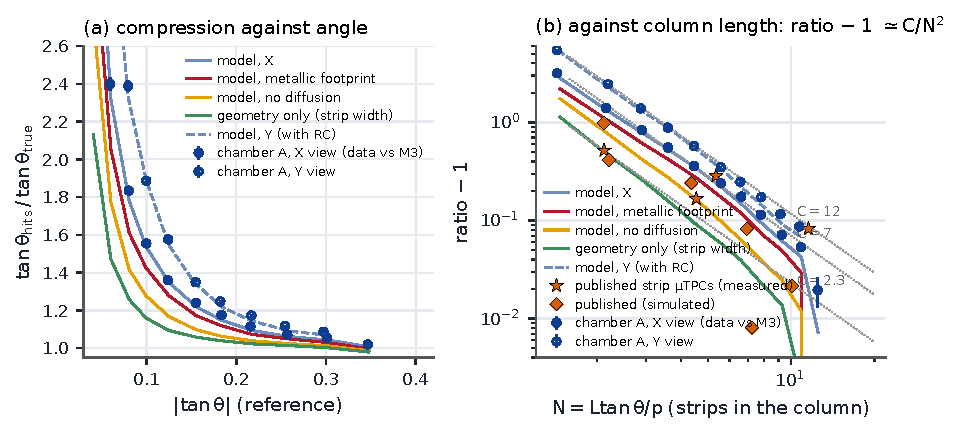
\includegraphics[width=\linewidth]{universal}
  \caption{(a) The median ratio of the hit-time angle to the reference angle against the reference angle, for the data of
  Run 1 (markers; filled X, open Y) and for the model arms (lines, exact truth). (b) The same as ratio $-1$ against the number of
  strips in the column, with the published strip-$\mu$TPC points converted from the quoted set and reconstructed angles with
  each chamber's gap and pitch (stars: measured; diamonds: circuit or gas-only simulations). Dotted lines: $C/N^2$ for $C = 2.3$
  (geometry), 7 (data X) and 12 (data Y).}
  \label{fig:universal}
\end{figure}

\begin{figure}[t]
  \centering
  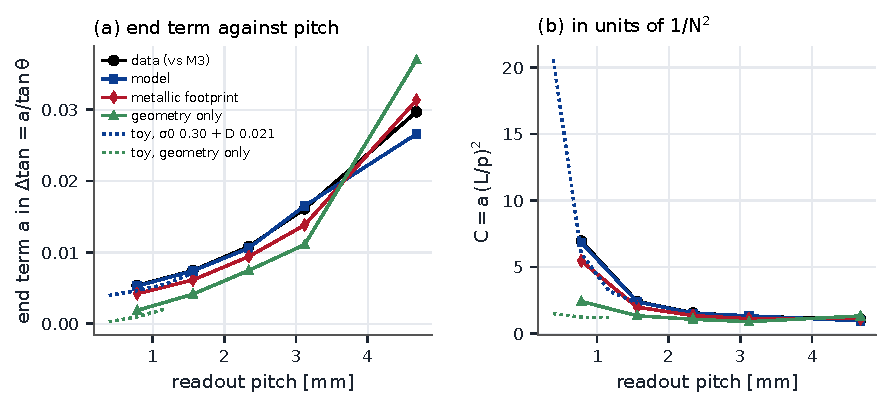
\includegraphics[width=\linewidth]{pitch_scan}
  \caption{The end term $a$ (left) and $C = a(L/p)^2$ (right) against the readout pitch, from summing adjacent strips of the
  same windows into readout elements of $k$ pitches; data against the reference, and the model arms. The toy (dotted) is the
  same scan with white noise.}
  \label{fig:pitch}
\end{figure}

The published points of \cref{fig:universal}b fall in the band spanned by the arms. Bortfeldt's measured \ang{10} point
($(\text{ratio}-1)N^2 = 2.3$) and Ntekas's gas-only simulation at \ang{10} (2.0) sit on the geometry line, Iodice's NSW chamber at
\ang{20} (3.4) and Bortfeldt's circuit model (3.9 to 4.7) between the geometry and the no-diffusion arms, and Flierl's GEM
(8.3 at \ang{15}, 10.8 at \ang{30}), whose diffusion at full drift is 0.8 of its pitch like ours, on the data line. The ordering follows
the lateral spread in units of the pitch, as \cref{eq:scaling} says it should; with diffusion coefficients assumed for the
LMU chambers and most-probable or mean angles quoted, this is a consistency check and not a measurement.

\subsection{Lateral sharing against drift depth}\label{sec:depth}

On tracks within \ang{0.5} of the drift direction ($|w| < \SI{3e-4}{mm/ns}$, so that the track moves less than a third of a pitch
over the gap) every sample of a strip's waveform belongs to a known drift time, smeared by the \SI{200}{ns} impulse response.
Stacking the waveforms of the five strips around the track at $t - t_0$ and dividing gives the neighbour shares against drift
depth (\cref{fig:depth}); the arms, regenerated on the same tracks and stacked the same way, carry the same smearing.

On the X view (569 planes) the first-neighbour share $(W_{-1} + W_{+1})/W_0$ is $0.50 \pm 0.02$ at $t_0$ and grows to 0.80 at
\SI{400}{ns} and $1.18 \pm 0.03$ at \SI{1000}{ns}. With the diffusion switched off the model's share is flat at 0.46 to 0.48: the growth
is drift diffusion, and its rate, read from the erf-fitted width of the five-strip pattern, is $d\sigma_{\rm eff}^2/dt =
\SI{3.5e-4}{mm^2/ns}$ against $4.2$ for the model's $D_p = 0.023$ and $3.2$ for $D_p = 0.020$: the data prefer $D_p \approx
\SI{0.021}{mm/\sqrt{ns}}$, $D_T \approx \SI{350}{\micro\metre\per\sqrt{cm}}$, 8\,\% below the fitted value and inside the Magboltz range for
this gas. The metallic arm starts at 0.27: without a same-time footprint of the model's size the mesh-end share is half the
data's, so a same-time share is required at the mesh, equivalent in the width metric to a Gaussian of \SIrange{0.33}{0.37}{mm}
on X. On Y (744 planes) the first-neighbour share grows to 2.0 by \SI{800}{ns} and the resistive spreading supplies most of
the growth (the arm without it reaches only 1.1); the mesh-end share is lower than on X ($0.49$ against $0.50$ with a model
that puts $0.60$ there), i.e.\ the same-time footprint along the resistive strips is narrower than across them, as it should be
if the footprint across the strips includes the equalisation of the avalanche charge over the \SI{550}{\micro\metre} strip
width~\cite{paperII}.

The second neighbours tell a different story. At $t_0$ their share is $0.049 \pm 0.004$ on X and $0.047 \pm 0.001$ on Y, about
2.4\,\% per side, where any Gaussian footprint of the fitted width gives less than 0.01 and the model 0.006; the kernels fitted
with a same-time second-neighbour term ($k_2 = 0.01$ to $0.02$) reproduce it (0.044 and 0.061). At depth the data's second-neighbour
share also exceeds every arm (0.27 against 0.24 for the model at \SI{1000}{ns} on X): the lateral distribution of the collected charge
has heavier tails than a Gaussian, at the mesh and at the cathode. A channel-map test~\cite{paperII} assigns most of the
mesh-end second-neighbour share to the electronics (1.34\,\% within a chip against $0.45 \pm 0.11$\,\% across a chip or connector
boundary on X); the first-neighbour share does not change across boundaries and is a property of the board.

\begin{figure}[t]
  \centering
  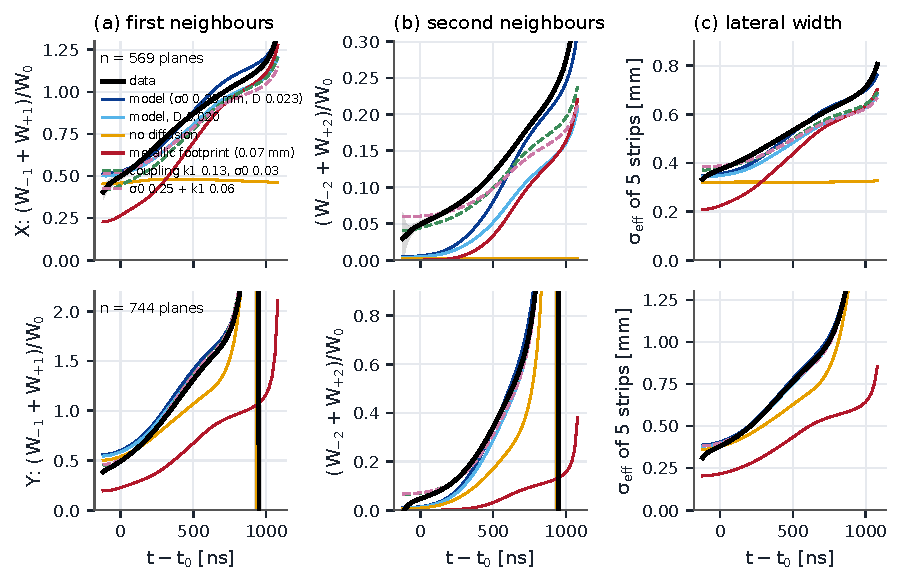
\includegraphics[width=\linewidth]{depth_sharing}
  \caption{Lateral sharing against drift depth on near-normal tracks ($|\tan\theta| < 0.008$), X (top) and Y (bottom): (a) the
  first-neighbour share, (b) the second-neighbour share, (c) the erf-fitted width of the five-strip pattern, all against the
  time after the mesh charge, for the data (black, with bootstrap band) and the model arms regenerated on the same tracks. The
  growth of (a) and (c) is drift diffusion (flat without it); the mesh-end values are the same-time share; the second neighbours
  at $t_0$ are a same-time floor that no Gaussian footprint produces.}
  \label{fig:depth}
\end{figure}

\subsection{Position in the strip: bounding a fixed coupling}\label{sec:phase}

A fixed nearest-neighbour coupling puts the same fraction on both neighbours wherever the charge lands in the strip; a Gaussian
footprint puts it on the nearer one. \Cref{fig:phase}a shows, at $t_0$ on the X view, the share of the neighbour on the side
the fitted track leans to (``near'') and of the other (``far'') in three bins of the track's position within the strip. Near
the centre the two are $0.37/0.22$; at the edge $0.84/0.10$. The Gaussian model reproduces the near side everywhere and the far
side near the centre, and under-predicts the far side at the edge (0.07 against $0.10 \pm 0.01$); a pure nearest-neighbour
coupling of 13\,\% with a \SI{33}{\micro\metre} footprint, the kernel that replaces $\sigma_0$ at equal waveform $\chi^2$, is too low on the
near side near the centre (0.33) and too high on the far side at the edge (0.13); a kernel with a \SI{0.25}{mm} footprint and a
6\,\% same-time term matches all three bins on both sides. On Y the data's far share at the edge (0.12) is below every model and
no same-time floor is required.

The phase is the fitted position, and a fit that leans towards the brighter neighbour could create a near/far asymmetry
in symmetric data. \Cref{fig:phase}b closes this on 2\,900 planes per view: windows regenerated with a known truth (a
\SI{0.32}{mm} Gaussian with no coupling, or the pure 13\,\% coupling with a \SI{33}{\micro\metre} footprint), fresh noise at the
strip's $\sigma$, and the track refitted with the production fitter exactly as for the data, are processed identically. The
refitted position scatters about the truth by \SI{0.007}{mm} (Gaussian truth) and \SI{0.07}{mm} (coupling truth), a tenth of
a pitch at most, and the near/far shares with the refitted and the true position agree within 0.01 in every bin; on the
pure-coupling truth the refit turns the symmetric $0.160/0.144$ of the centre bin into $0.174/0.138$, a lean that falls far short
of the data's $0.205/0.124$. The test is therefore sound. On X the data's far share is $0.124$ at the centre and then flat at
$0.060$ to $0.067$ from a quarter pitch outward, where the Gaussian truth falls from 0.167 to 0.040 and the pure coupling stays
at 0.13: the data have a floor, and it is half the published coupling. On Y the floor is $0.10$ against a Gaussian's 0.07 and the
coupling's 0.13, while the centre bin ($0.216/0.159$) lies below the Gaussian's $0.279/0.209$: the same-time footprint along the
resistive strips is narrower than the fitted \SI{0.28}{mm} with a floor on top. In both views the same-time share is a narrow core
plus a flat few-per-cent floor, the shape of the kernels fitted with a footprint and a same-time term ($\sigma_0 = \SI{0.25}{mm}$ with
$k_1 = 0.06$ on X; \SI{0.12}{mm} with $0.09$ on Y~\cite{paperII}). A fixed nearest-neighbour coupling on chamber A is thus bounded at
about 6\,\% (X) to 10\,\% (Y) per neighbour, a factor two to five below the 15 to 30\,\% of the strip-$\mu$TPC literature, and
consistent with the published fraction that a floating resistive strip images onto the adjacent readout column for this stack-up
($\sim 1\,\%$ per side~\cite{paperII}) only if a further same-time process is present. Its physical origin is not identified. For
the angle it does not matter: the floor's variance is what the ghost strips see, and the forward model carries it as part of
$\sigma_0$.

\begin{figure}[t]
  \centering
  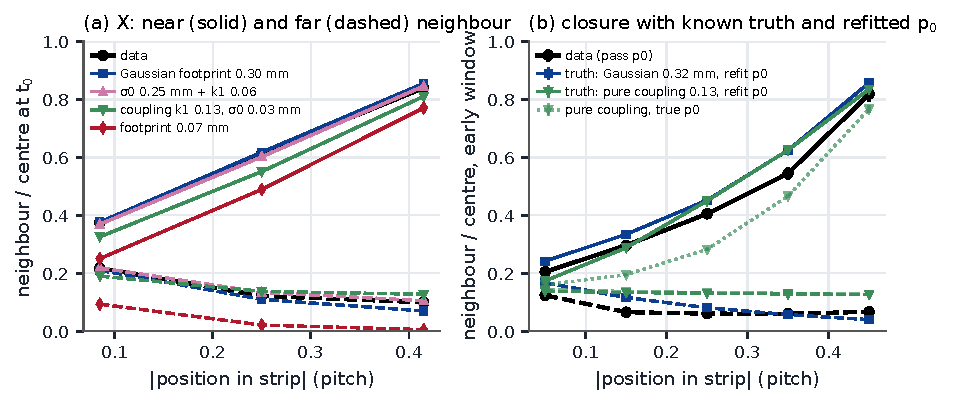
\includegraphics[width=\linewidth]{phase}
  \caption{(a) Near (solid) and far (dashed) neighbour share at $t_0$ on X against the track's position within the centre
  strip, data and models regenerated on the same tracks with the fitted position. (b) The closure: the same quantity on
  windows of known truth, with the track position refitted by the production fitter.}
  \label{fig:phase}
\end{figure}

\subsection{Ghost strips}\label{sec:ghosts}

The end effect lives in the strips beyond the column. Counting the strips with a hit whose centre lies more than half a
pitch outside the track's projection (\cref{fig:ghosts}), the data have 3.4 ghosts per plane on X at $|\tan\theta| = 0.08$--$0.15$
against 2.6 in the model with the same noise, and the excess is at the mesh end (1.57 against 0.82 per plane; the cathode end
agrees, 1.82 against 1.75). On Y the data have 5.5 ghosts per plane against 5.4 and the two ends agree within 0.3. The
mesh-end excess on X is the same-time floor of \cref{sec:depth} seen from the other side: charge that no Gaussian of the
fitted width brings to the second strip, at the earliest times, where it rotates the ladder most. It is the part of chamber
A's compression that the model does not describe, and the reason the arms with the real residual sit one unit of $C$ above
the toy.

\begin{figure}[t]
  \centering
  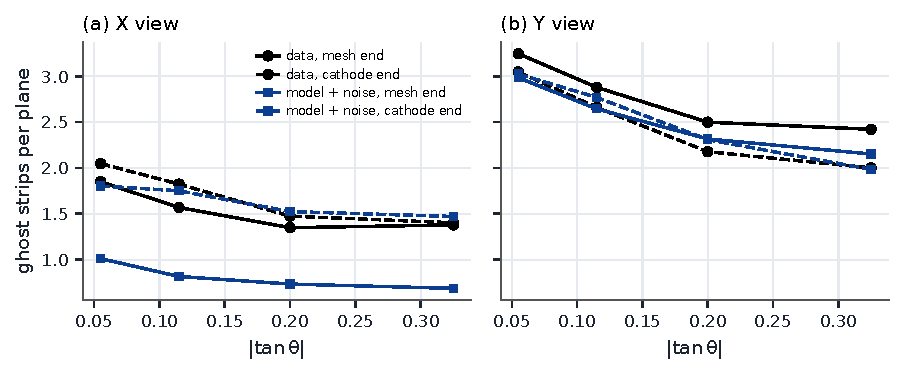
\includegraphics[width=0.8\linewidth]{ghosts}
  \caption{Ghost strips per plane (hits more than half a pitch beyond the track's projection), at the mesh end (solid) and the
  cathode end (dashed), data against the model with the same noise, Run 1.}
  \label{fig:ghosts}
\end{figure}
